\section{Electrostatic Analysis}

The electric and magnetic fields are completely decoupled (the field induction cease to exist). E-field and H-field exist independent from each other. \\

Since $\frac{\partial}{\partial t} = 0$ Maxwell Equations (\ref{eq:MaxwellDiff1_1}), (\ref{eq:MaxwellDiff1_4}), (\ref{eq:MaxwellDiff2_1}) and (\ref{eq:MaxwellDiff2_4}) can be written as

\begin{tabular}{ll}
	\(\displaystyle \nabla \cdot \vec{D} = \rho \) & \(\displaystyle \nabla \cdot \vec{E} = \frac{\rho}{\varepsilon} \) \\
	\(\displaystyle \nabla \times \vec{E} = 0 \) \hspace{2cm} & \(\displaystyle \nabla \times \vec{E} = 0 \) .
\end{tabular}

Since the curl of the electric field is always equal to zero, the electric field can be described as agradient of the electric scalar potential
\begin{equation*}
	\vec{E} = -\nabla \varphi \rightarrow \underbrace{\nabla \cdot \left(\varepsilon \nabla \varphi\right) = -\rho}_{\text{quasi-Poisson equation}} \rightarrow \nabla \cdot \nabla \varphi = -\frac{\rho}{\varepsilon} \rightarrow \underbrace{\Delta \varphi = -\frac{\rho}{\varepsilon}}_{\text{Poisson equation if $\varepsilon$ is everywhere equal}}
\end{equation*}
Thus, in a homogeous material the electric field is a solution of the following Poisson
\begin{equation*}
	\frac{\partial \varphi}{\partial x^2} + \frac{\partial \varphi}{\partial y^2} +\frac{\partial \varphi}{\partial z^2} = \Delta \varphi = - \frac{\rho}{\varepsilon}
\end{equation*}
or the following Laplace equation
\begin{equation*}
	\frac{\partial \varphi}{\partial x^2} + \frac{\partial \varphi}{\partial y^2} +\frac{\partial \varphi}{\partial z^2} = \Delta \varphi = 0
\end{equation*}
written in Cartesian coordinate. {\tiny \texttt{other coordinates in Bronstein: P.723}}

\textbf{\\ Boundary Value Problem (BVP)\\}
\begin{minipage}[lt]{11cm}
	\begin{tabular}{l}
		\(\displaystyle \frac{\partial \varphi}{\partial x^2} + \frac{\partial \varphi}{\partial y^2} +\frac{\partial \varphi}{\partial z^2} = \Delta \varphi = - \frac{\rho}{\varepsilon}, \textrm{ in } \Omega\) \\
		\(\displaystyle \varphi = 0, \textrm{ over } \partial_{D2} \Omega \) \\
		\(\displaystyle \varphi = U, \textrm{ over } \partial_{D1} \Omega \rightarrow \) Dirichlet Boundary \\
		\(\displaystyle \frac{\partial \varphi}{\partial n} = 0, \textrm{ over } \partial_{N} \Omega \rightarrow \) Neumann Boundary \\	
		Definition Normalenableitung: \(\displaystyle \vec{n} \cdot \left(\nabla \varphi\right) = \frac{\partial \varphi}{\partial n}\)	
	\end{tabular}
\end{minipage}
\begin{minipage}[rt]{8cm}
	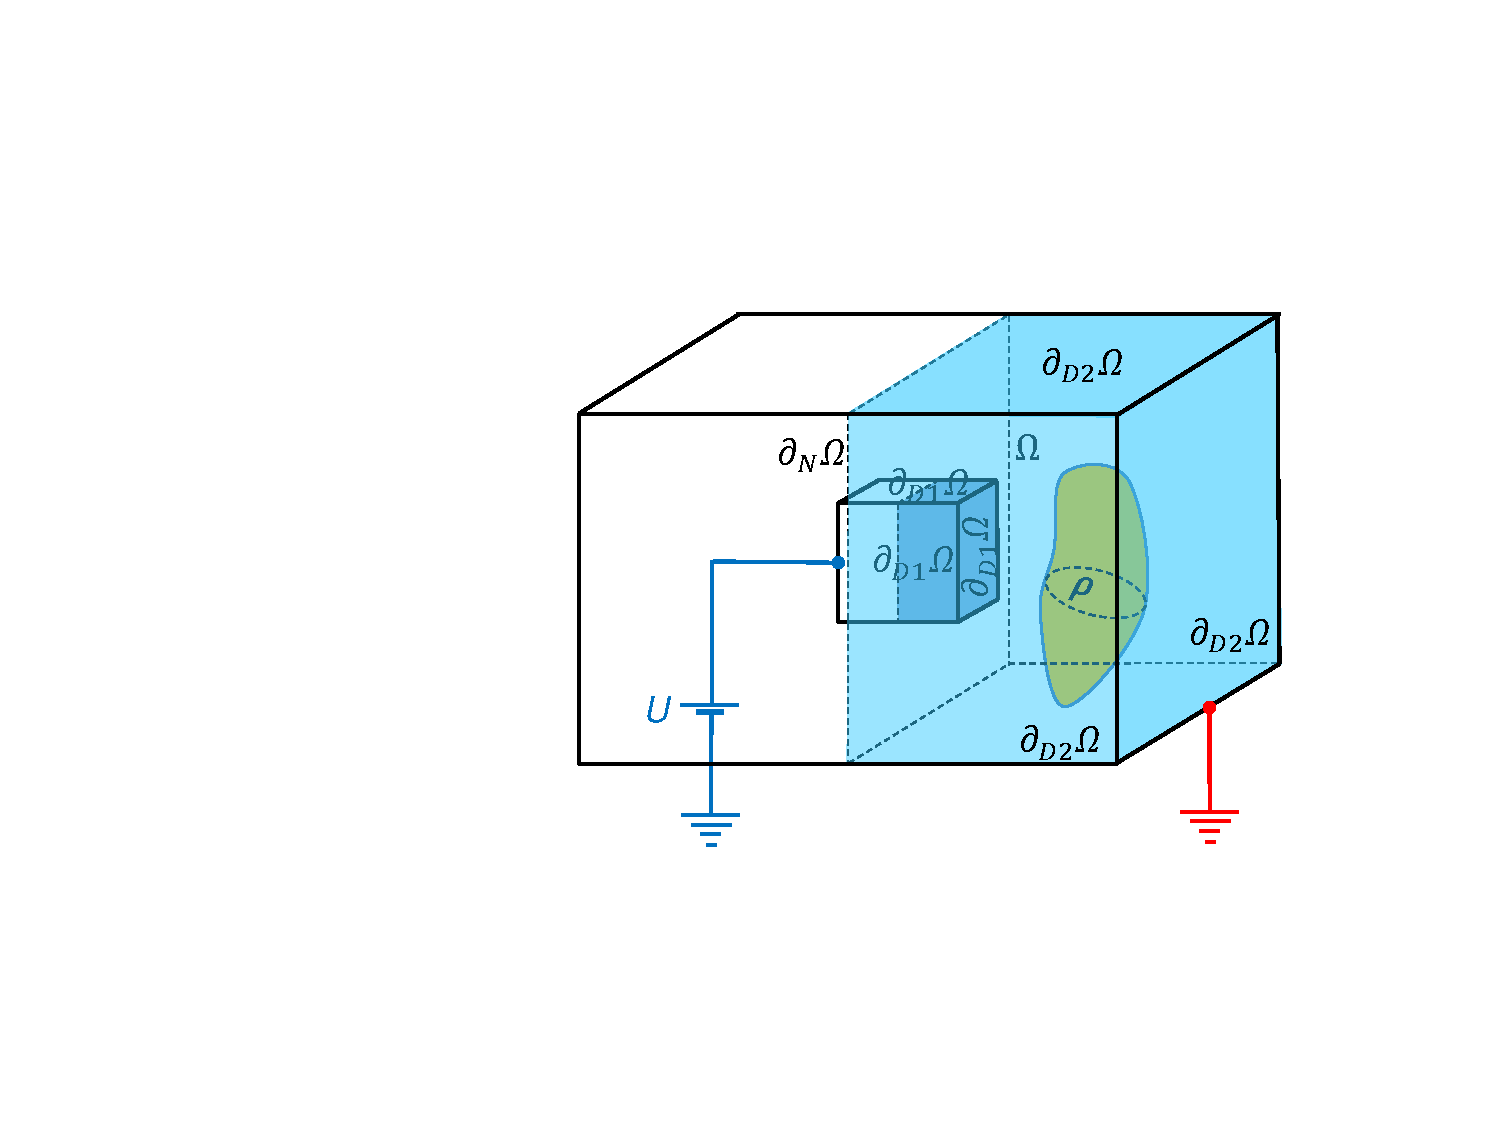
\includegraphics[width=.8\textwidth]{./images/BVP_electrostatic.pdf}
\end{minipage}